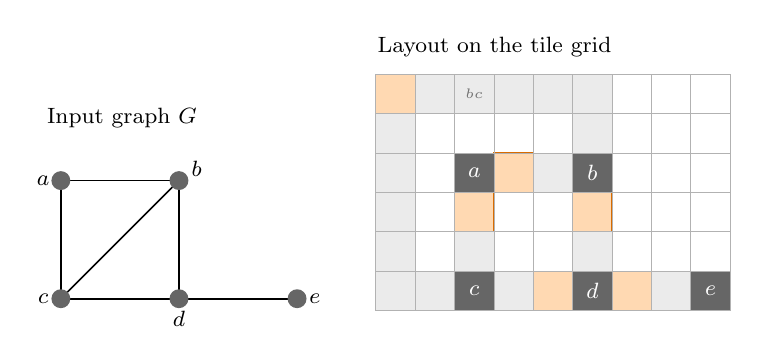
\begin{tikzpicture}[x=0.5cm,y=0.5cm]
  \tikzstyle{labelstyle}=[font=\footnotesize]
  \tikzstyle{tinylabel}=[font=\tiny]
  \tikzstyle{guidestyle}=[line width=0.3pt, draw=black!30]
  \tikzstyle{pathtile}=[draw=black!30, fill=black!8, line width=0.3pt]
  \tikzstyle{verttile}=[draw=black!70, fill=black!60, line width=0.3pt]
  \tikzstyle{midtile}=[draw=orange!85!black, fill=orange!30, line width=0.45pt]

  % ---------- (a) input graph ----------
  \begin{scope}[shift={(0.5,2.3)}]
    \node[labelstyle, anchor=west] at (-0.6,4.6) {Input graph $G$};
    \draw[line width=0.6pt] (0,3) -- (3,3);
    \draw[line width=0.6pt] (0,3) -- (0,0);
    \draw[line width=0.6pt] (3,3) -- (0,0);
    \draw[line width=0.6pt] (3,3) -- (3,0);
    \draw[line width=0.6pt] (0,0) -- (3,0);
    \draw[line width=0.6pt] (3,0) -- (6,0);
    \foreach \x/\y/\n/\ax/\ay in {0/3/a/-0.45/0, 3/3/b/0.45/0.3, 0/0/c/-0.45/0, 3/0/d/0/-0.5, 6/0/e/0.45/0} {
      \fill[black!60] (\x,\y) circle (0.24);
      \node[labelstyle] at (\x+\ax,\y+\ay) {$\n$};
    }
  \end{scope}

  % ---------- (b) layout on the tile grid ----------
  \begin{scope}[shift={(7.5,0)}]
    \node[labelstyle, anchor=west] at (0.8,8.7) {Layout on the tile grid};
    % edge-path tiles
    \foreach \x/\y in {5/5, 3/3, 6/3, 4/2, 8/2,
                       6/6,6/7,5/7,4/7,3/7,2/7,1/6,1/5,1/4,1/3,1/2,2/2} {
      \draw[pathtile] (\x,\y) rectangle ++(1,1);
    }
    \node[tinylabel, text=black!55] at (3.5,7.5) {$bc$};
    % midpoint tiles
    \foreach \x/\y in {4/5, 3/4, 6/4, 5/2, 7/2, 1/7} {
      \draw[midtile] (\x,\y) rectangle ++(1,1);
    }
    % vertex tiles
    \foreach \x/\y/\n in {3/5/a, 6/5/b, 3/2/c, 6/2/d, 9/2/e} {
      \draw[verttile] (\x,\y) rectangle ++(1,1);
      \node[labelstyle, text=white] at (\x+0.5,\y+0.5) {$\n$};
    }
    \draw[guidestyle, step=1] (1,2) grid (10,8);
  \end{scope}
\end{tikzpicture}
